
\chapter{Resultados}
En este capítulo se muestran todos los resultados obtenidos del desarrollo y ejecución del trabajo descrito en el capítulo anterior. Una vez se ha mostrado la manera con la que sea aborda la problemática y las distintas técnicas utilizadas para ello, a continuación, se muestran los distintos resultados que se han obtenido de los distintos procesos desarrollados.

\section{Definición de experimentos realizados.}\label{sec:definicion_experimentos}

Para guiar al lector en los experimentos rea\begin{subfigure}[b]{0.60\lin\begi\begin{figure}[h!]
\centering
 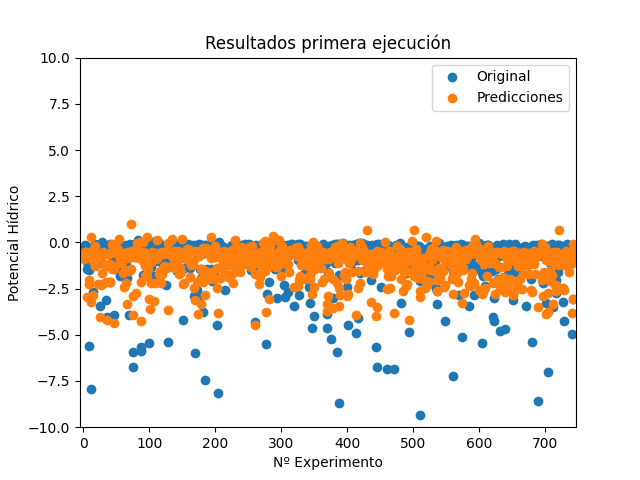
\includegraphics[width=.8\linewidth]{images/Prediccion.png}
\caption{Predicción del individuo 0101000010010}
\label{fig:prediccion_final}
\end{figure}re}[h!]
\centering
 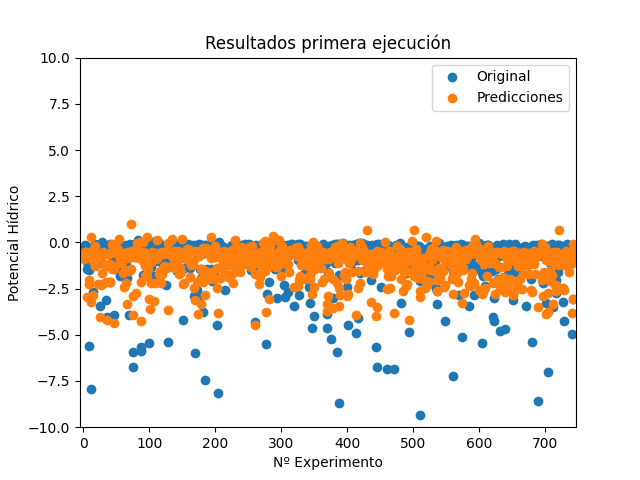
\includegraphics[width=.8\linewidth]{images/Prediccion.png}
\caption{Predicción del individuo 0101000010010}
\label{fig:prediccion_individuo}
\end{figure}}
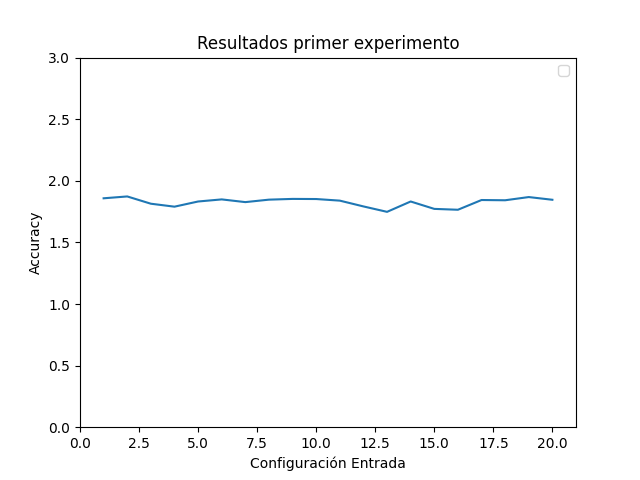
\includegraphics[width=.7\linewidth]{images/resultSecondEval.png}
\caption{Accuracy por ejecución para experimento 3}
\label{fig:accuracy_experiment3}
\end{subfigure}in{subfigure}[b]{0.60\linewidth}
 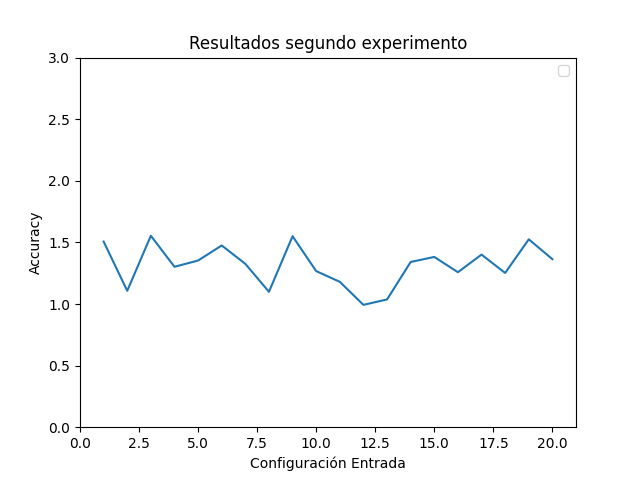
\includegraphics[width=.7\linewidth]{images/resultFourthEval.png}
\caption{Accuracy por ejecución para experimento 4}
\label{fig:accuracy_experiment4}
\end{subfigure}s se detallan a continuación:

\begin{itemize}
    \item Determinación de épocas idóneas para la red neuronal: En este primer paso se determina el número de épocas que, \textit{a priori}, permite la mejor optimización del modelo.
    \item Aplicación de algoritmo genético para determinar la mejor combinación de parámetros de entrada para la red neuronal será presentado desde 2 enfoques diferentes mostrados a continuación:
    \newpage
    \begin{itemize}
        \item Enfoque 1: Fitness:
\[
\centering
 fitness = accuracy \cdot N Ones
\]
    
    \noindent donde el accuracy de la red neuronal se multiplica por el número de unos, para intentar minimizar el número de sensores utilizados.
    
        \item Enfoque 2: Fitness:
        
\begin{center}
\begin{algorithmic}
\If{$N Ones\geq 3$} 
    \State $fitness = accuracy \cdot N Ones$
\Else
    \State $fitness = accuracy \cdot 3 \cdot N Ones$
\EndIf
\end{algorithmic}
\end{center}


    \noindent donde se sigue el mismo criterio anterior pero se busca que el algoritmo genético utilice al menos 3 sensores.
    
    \end{itemize}

\end{itemize}


Ambos enfoques son ejecutados con dos combinaciones de parámetros de entrada diferentes:

\begin{itemize}
    \item Utilización de 7 sensores.
    \item Utilización de 7 sensores más las variables climáticas, total 13 variables de entrada.
\end{itemize}


En resumen, se realizarán los siguientes experimentos:
\begin{itemize}
    \item \textbf{Experimento 1}: 7 variables de entrada - Enfoque 1.
    \item \textbf{Experimento 2}: 13 variables de entrada - Enfoque 1.
    \item \textbf{Experimento 3}: 7 variables de entrada - Enfoque 2.
    \item \textbf{Experimento 4}: 13 variables de entrada - Enfoque 2.
\end{itemize}


\section{Determinación de épocas idóneas para la red neuronal}\label{sec:epocas}


Como inicio del desarrollo de los resultados, se obtienen de manera independiente ciertos resultados de la red neuronal para poder observar como reacciona la red ante el uso de ciertos datos de entrada y el no uso de los mismos. Se estudia la evolución de la red en función a las épocas asignadas a ésta y así poder observar como mejora o empeora esta en función al número de ciclos que la red realiza. Con ello se intenta determinar las épocas idóneas para la red, no ejecutando menos épocas de las necesarias y tampoco un número elevado el cual no sería necesario ya que la red no evoluciona favorablemente a un número alto de épocas, utilizando un tiempo innecesario en cada cálculo.

Posteriormente, y una vez analizado independientemente la red neuronal, se buscan las mejores configuraciones de datos de entrada para la red mediante el uso del algoritmo genético descrito en capítulos anteriores.


En primer lugar, de manera aleatoria se seleccionan ciertas configuraciones de entrada que se presentan a continuación:

\begin{itemize}
    \item 1010101
    \item 1111111
    \item 0000100
    \item 1010101010101
    \item 1111111111111
    \item 0000100000110
\end{itemize}

Para saber qué sensores y datos medioambientales son los utilizados en las dos representaciones de los individuos consultar el punto \ref{PuntoIndividuo}. Como puede observarse, se utilizan configuraciones de individuos completamente a \textit{unos (1)} para identificar el uso completo de todos los sensores y/o variables de clima.


Se obtiene el accuracy de estas configuraciones en función al número de épocas que va desde 10, incrementando en 10 épocas, hasta llegar a 500 épocas como máximo. La figura \ref{fig:accuracy_epocas_first_eval} muestra los resultados de accuracy de cada configuración seleccionada.

\begin{figure}[h!]
\begin{subfigure}[b]{0.47\linewidth}
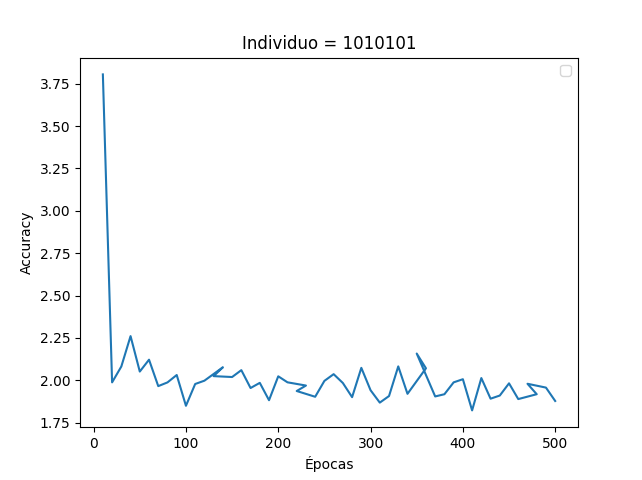
\includegraphics[width=.7\linewidth]{images/Figure_1.png}
\caption{Individuo = 1010101}
\label{fig:individuo_1010101}
\end{subfigure}
\begin{subfigure}[b]{0.47\linewidth}
 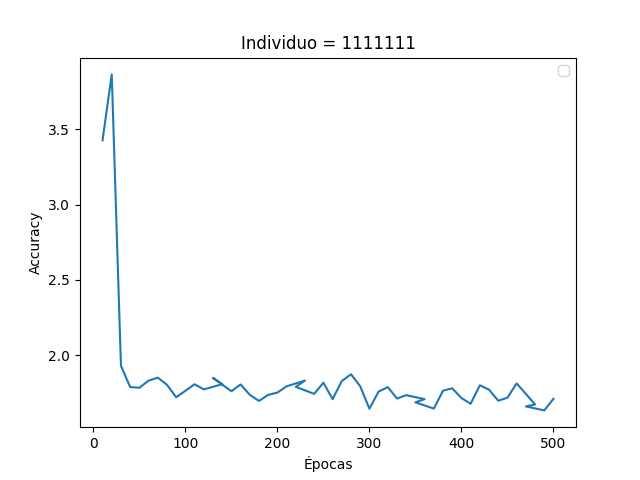
\includegraphics[width=.7\linewidth]{images/Figure_2.png}
\caption{Individuo = 1111111}
\label{fig:individuo_1111111}
\end{subfigure}
\begin{subfigure}[b]{0.47\linewidth}
 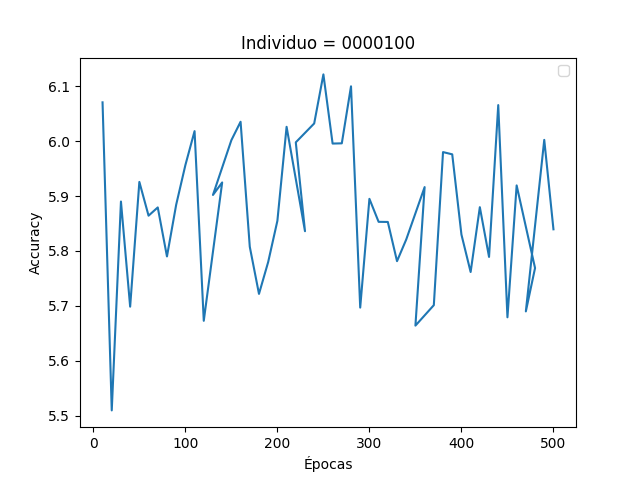
\includegraphics[width=.7\linewidth]{images/Figure_3.png}
\caption{Individuo = 0000100}
\label{fig:individuo_0000100}
\end{subfigure}
\begin{subfigure}[b]{0.47\linewidth}
 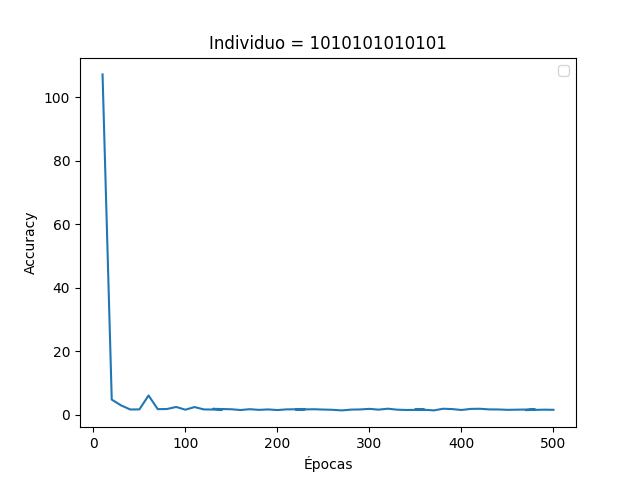
\includegraphics[width=.7\linewidth]{images/Figure_4.png}
\caption{Individuo = 1010101010101}
\label{fig:individuo_1010101010101}
\end{subfigure}
\begin{subfigure}[b]{0.47\linewidth}
 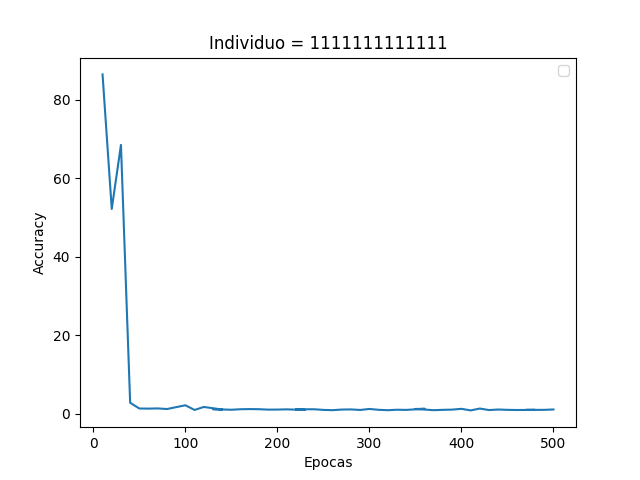
\includegraphics[width=.7\linewidth]{images/Figure_5.png}
\caption{Individuo = 1111111111111}
\label{fig:individuo_1111111111111}
\end{subfigure}
\begin{subfigure}[b]{0.47\linewidth}
 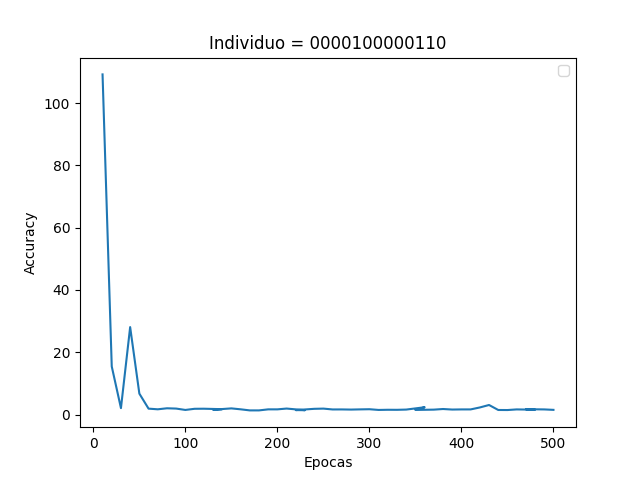
\includegraphics[width=.7\linewidth]{images/Figure_6.png}
\caption{Individuo = 0000100000110}
\label{fig:individuo_0000100000110}
\end{subfigure}
\caption{Representación accuracy en función al número de épocas}
\label{fig:accuracy_epocas_first_eval}
\end{figure}

\newpage
Se puede observar como la opción donde el individuo tiene un valor de 0000100 los resultados obtenidos rondan entre el 5.5\% y 6.1\% de accuracy. A medida que las épocas aumentan no mejora y se mantiene en el rango comentado. Ciertas configuraciones pueden obtener variables de entrada activas que no supongan ningún tipo de mejora, pero su combinación con otras variables más precisas hará que su peor rendimiento de forma independiente mejore en combinación con otras variables seleccionadas por el algoritmo genético. Cuando estas variables más significativas no son incorporadas en el individuo, se muestra su debilidad, obteniendo malos resultados, independientemente del número de épocas con el que configuremos la red en su entrenamiento.. 

Mientras tanto en el resto de pruebas realizadas llega un momento donde el accuracy rara vez supera el 2\%. 


Se puede observar cómo en casi todas las opciones el accuracy desciende de una manera considerable a medida que sus épocas crecen. Observando los resultados se puede deducir que el número de épocas de la red estaría entre 50 y 150, por lo que establecemos en el umbral intermedio de 100 épocas, ya que la mejora no es significativa en un número mayor, a diferencia del tiempo de evaluación del individuo que si aumenta considerablemente. Puede observarse la evolución de los experimentos iniciales en las tablas \ref{tab:accuracy},\ref{tab:accuracy2}:


\begin{table}[h!]
    \centering
    \begin{tabular}{|c|c|}
        \hline
        \textbf{Época} & \textbf{Accuracy} \\
        \hline
        50 & 1.621 \\
        \hline
        60 & 6.007 \\
        \hline
        70 & 1.700 \\
        \hline
        80 & 1.745 \\
        \hline
        90 & 2.391 \\
        \hline
        100 & 1.527 \\
        \hline
        110 & 2.364 \\
        \hline
        120 & 1.618 \\
        \hline
        130 & 1.536 \\
        \hline
        140 & 1.801 \\
        \hline
        150 & 1.669 \\
        \hline
    \end{tabular}
    \caption{Individuo = 1010101}
    \label{tab:accuracy}
\end{table}


\begin{table}[h!]
    \centering
    \begin{tabular}{|c|c|}
        \hline
        \textbf{Época} & \textbf{Accuracy} \\
        \hline
        50 & 6.715 \\
        \hline
        60 & 1.892 \\
        \hline
        70 & 1.681 \\
        \hline
        80 & 2.007 \\
        \hline
        90 & 1.913 \\
        \hline
        100 & 1.475 \\
        \hline
        110 & 1.843 \\
        \hline
        120 & 1.867 \\
        \hline
        130 & 1.551 \\
        \hline
        140 & 1.722 \\
        \hline
        150 & 1.973 \\
        \hline
    \end{tabular}
    \caption{Individuo = 1010101010101}
    \label{tab:accuracy2}
\end{table}

Los resultados de la red son más precisos si las épocas crecen, llegando a un número de épocas en las cuales la mejora ya no es significativa. A partir de la época 100, de forma general, es en donde los resultados tienden a converger, variando muy poco y en ocasiones experimentando algún repunte de malos resultados, algo a no tener muy en cuenta dada la naturaleza probabilística de la red neuronal la cual con las mismas características puede arrojar resultados bueno y posteriormente sin variar nada en la red dar peores resultados.

Una vez finalizado el análisis de los resultados, se puede afirmar la existencia de  configuraciones de entrada para la red las cuales obtengan el valor del potencial hídrico con un accuracy menor al 2\% en función a los datos otorgados por los sensores y los datos medioambientales. Se puede concretar además que de una manera aproximada a partir de la época 100 se obtienen resultados satisfactorios y estables en el tiempo. 



\section{Análisis de resultados con Algoritmo Genético}

Una vez analizado los resultados de la red de manera independiente, se buscan las mejores configuraciones de entrada para esta. Para ello se llevan a cabo los 4 experimentos detallados en la sección \ref{sec:definicion_experimentos}, repetidos con diferentes combinaciones de los operadores genéticos, esto es: diferentes tipos de selección (Ranking, Truncado, Ruleta, Torneo), tipo de cruce (1 punto, 2 puntos, uniforme), tipo de remplazamiento de la población (generacional, estacionario) y elitismo (0, 1, 2 individuos). Todas las combinaciones cuentan con un total de 50 individuos para los experimentos 1 y 3 (uso de 7 variables de entrada) y 100 individuos para los experimentos 2 y 4 (uso de 13 variables de entradas), en todos los experimentos el número de generaciones se fija en 3.

Tal y como se demuestra en la sección \ref{sec:epocas} el número de épocas para la optimización de la red neuronal es de 100. 

Para cada uno de los 4 experimentos se realizan 20 repeticiones del mismo con diferentes combinaciones de los operadores genéticos, tal y como se muestran en las tablas \ref{tab:experimento1}, \ref{tab:experimento2}, \ref{tab:experimento3}, \ref{tab:experimento4}


\subsection{Experimento 1}

Recordamos la configuración del experimento 1: uso de 7 variables de entrada y enfoque 1 para el cálculo de la fitness. Con este experimento se pretende reducir el número de sensores utilizados, por lo que se penaliza el uso de los mismos.

La tabla \ref{tab:experimento1} muestra los resultados de las 20 combinaciones de operadores genéticos para determinas una la mejor solución y mejor combinación de parámetros. Puede observarse claramente que las soluciones tienen a utilizar un número muy bajo de sensores, lo que penaliza mucho el accuracy con respecto a utilizar todos los sensores disponibles (el peor de los escenarios posibles)


\begin{filecontents*}{result_table_first.csv}
idindiv,configuracion,accuracy,fitness,elitismo,selec,cruce,reemplazamiento
1,0000001,2.039,2.039,2,Ranking,1 punto,Estacionario
2,0000001,1.981,1.981,2,Ranking,Uniforme,Generacional
3,0000001,2.057,2.057,2,Ranking,Uniforme,Generacional
4,0000001,1.995,1.995,1,Ranking,1 punto,Generacional
5,0000001,2.042,2.042,0,Truncado,Uniforme,Estacionario
6,0000001,1.925,1.925,0,Truncado,Uniforme,Estacionario
7,0000001,1.944,1.944,0,Truncado,Uniforme,Generacional
8,0000001,2.007,2.007,0,Truncado,Uniforme,Generacional
9,0000001,1.909,1.909,1,Truncado,1 punto,Generacional
10,0000001,1.970,1.970,1,Ruleta,1 punto,Estacionario
11,1000001,1.844,3.688,2,Ruleta,1 punto,Generacional
12,0000001,1.845,1.845,2,Ruleta,1 punto,Generacional
13,1000001,1.992,3.984,2,Ruleta,Uniforme,Generacional
14,1000001,1.913,3.826,0,Ruleta,Uniforme,Generacional
15,1101011,1.846,9.231,0,Torneo,1 punto,Estacionario
16,0010001,1.969,3.9391,2,Torneo,1 punto,Estacionario
17,0000001,1.966,1.966,1,Torneo,1 punto,Estacionario
18,0000011,1.901,3.802,2,Torneo,1 punto,Estacionario
19,1101111,1.866,11.199,0,Torneo,1 punto,Generacional
20,0000101,1.924,3.848,1,Torneo,Uniforme,Estacionario
\end{filecontents*}



\begin{table}[h]
    \centering
    \begin{adjustbox}{max width=\textwidth}
    \begin{tabular}{|c|c|c|c|c|c|c|c|}%
    \hline
    \bfseries Id ejecución & \bfseries Mejor Individuo & \bfseries Accuracy & \bfseries Fitness & \bfseries Elitismo & \bfseries Selección & \bfseries Cruce & \bfseries Reemplazamiento % specify table head
    \csvreader[head to column names]{result_table_first.csv}{}% use head of csv as column names
    {\\\hline \idindiv & \configuracion & \accuracy & \fitness & \elitismo & \selec & \cruce & \reemplazamiento} % specify your coloumns here
    \\
    \hline
    \end{tabular}
    \end{adjustbox}
    \caption{Soluciones \textbf{Experimento 1}}
    \label{tab:experimento1}
\end{table}




\subsection{Experimento 2}


Recordamos la configuración del experimento 2: uso de 13 variables de entrada y enfoque 1 para el cálculo de la fitness. Con este experimento se pretende reducir el número de sensores utilizados junto con variables climáticas, por lo que se penaliza el uso de los mismos.

La tabla \ref{tab:experimento2} muestra los resultados de las 20 combinaciones de operadores genéticos para determinas una la mejor solución y mejor combinación de parámetros. Puede observarse claramente que las soluciones tienen a utilizar un número muy bajo de sensores, lo que penaliza mucho el accuracy con respecto a utilizar todos los sensores disponibles (el peor de los escenarios posibles)





\begin{filecontents*}{result_table_third.csv}
idindiv,configuracion,accuracy,fitness,elitismo,selec,cruce,reemplazamiento
1,0000010000000,1.622,1.622,2,Ranking,1 punto,Estacionario
2,1000000000000,2.060,2.0600,2,Ranking,1 punto,Estacionario
3,0010000000000,1.629,1.629,2,Ranking,2 puntos,Estacionario
4,0000000010000,1.674,1.674,0,Ranking,2 puntos,Estacionario
5,0000010000000,1.447,1.447,0,Ranking,Uniforme,Estacionario
6,0001000000000,1.603,1.603,0,Ranking,1 punto,Generacional
7,0000010001000,1.333,2.667,2,Ranking,2 puntos,Generacional
8,0000000000001,2.015,2.015,0,Ranking,2 puntos,Generacional
9,1000000000000,2.128,2.128,0,Ruleta,1 punto,Estacionario
10,0001000010000,1.600,3.201,1,Ruleta,2 puntos,Generacional
11,0001000000000,1.823,1.823,2,Ruleta,2 puntos,Generacional
12,0100001000000,1.869,3.739,0,Ruleta,Uniforme,Generacional
13,0001001000001,1.469,4.408,2,Torneo,1 punto,Estacionario
14,0110101110110,0.964,7.718,0,Torneo,2 puntos,Estacionario
15,0001001100000,1.424,4.273,1,Torneo,2 puntos,Estacionario
16,0000010010000,1.479,2.959,2,Torneo,Uniforme,Estacionario
17,0000000010010,1.831,3.663,2,Torneo,1 punto,Generacional
18,1001110001000,1.537,7.688,0,Torneo,2 puntos,Generacional
19,0000000000010,2.378,2.378,2,Torneo,2 puntos,Generacional
20,0011111000111,1.159,9.275,0,Torneo,Uniforme,Generacional

\end{filecontents*}




\begin{table}[H]
    \centering
    \begin{adjustbox}{max width=\textwidth}
    \begin{tabular}{|c|c|c|c|c|c|c|c|}%
    \hline
   \bfseries Id Ejecución & \bfseries Mejor Individuo & \bfseries Accuracy & \bfseries Fitness & \bfseries Elitismo & \bfseries Selección & \bfseries Cruce & \bfseries Reemplazamiento% specify table head
    \csvreader[head to column names]{result_table_third.csv}{}% use head of csv as column names
    {\\\hline \idindiv & \configuracion\ & \accuracy & \fitness & \elitismo & \selec & \cruce & \reemplazamiento} % specify your coloumns here
    \\
    \hline
    \end{tabular}
    \end{adjustbox}
    \caption{Soluciones \textbf{Experimento 2}}
    \label{tab:experimento2}
\end{table}




En la figura \ref{fig:ejecuciones_exp1_exp2} representa la fitness en cada una de las 20 ejecuciones realizadas para los experimentos 1 y 2, donde el eje X representa el número de ejecución y el Eje Y el accuracy alcanzado en esa ejecución. Puede observarse que el experimento 1 hay poca variación, no así en el experimento 2 que es más sensible a la combinación de variables de entrada seleccionadas por el algoritmo genético.


\begin{figure}[H] 
\begin{subfigure}[b]{0.60\linewidth}
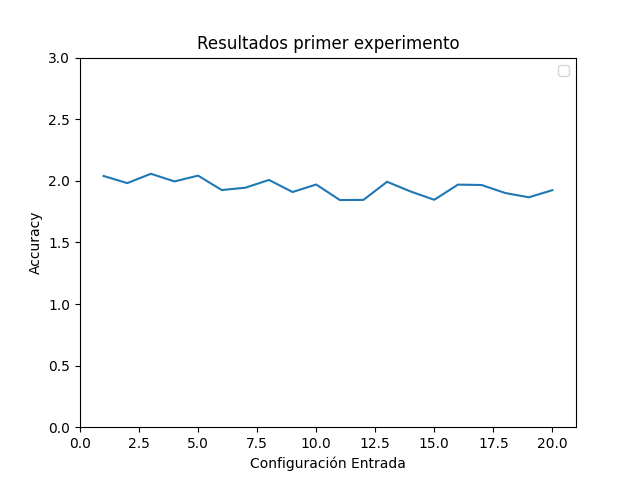
\includegraphics[width=.7\linewidth]{images/resultFirstEval.png}
\caption{Accuracy por ejecución para experimento 1}
\label{fig:accuracy_experiment1}
\end{subfigure}
\begin{subfigure}[b]{0.60\linewidth}
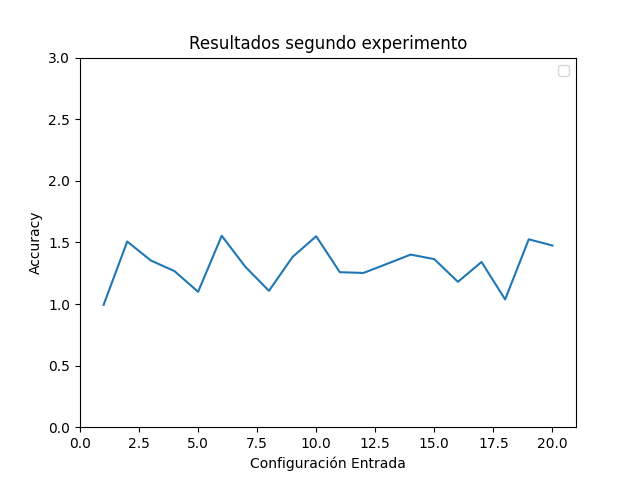
\includegraphics[width=.7\linewidth]{images/resultThirdEval.png}
\caption{Accuracy por ejecución para experimento 2}
\label{fig:accuracy_experiment2}
\end{subfigure}
\caption{Accuracy experimentos 1 y 2 (Enfoque 1)}
\label{fig:ejecuciones_exp1_exp2}
\end{figure}



Se puede observar como los resultados del \textbf{experimento 1}, independientemente de la combinación de operadores genéticos utilizados, en su mayoría la mejor solución encontrada es para el individuo \textit{0000001}. Esta arroja unos resultados bastante satisfactorios donde el accuracy de la red se aproxima al 2. Con esto se puede llegar a la conclusión que cuando al menos esta variable concreta este activa en otro tipo de configuraciones la posibilidad de obtener buenos resultados es bastante alta. Esto no implica que esta configuración sea la mejor a pesar de ser la más repetida dentro del conjunto de soluciones. Podemos ver como también se pueden ver otros tipos de soluciones donde el accuracy obtenido en la red es mejor que en la solución comentada como puede ser la configuración con mejor individuo \textit{1000001}, obtiene resultados aún menores, por debajo del un accuracy con valor 2, se traduce en peor fitness debido a la penalización por el uso de más sensores en otras soluciones.

Por otro lado, analizando las soluciones otorgadas por el experimento 2, podemos observar como el abanico de soluciones es mucho mayor que en el otro caso, dando un conjunto más amplio de distintos tipos de soluciones con resultados que exceptuando algunos casos no superan el accuracy de 2. De entre todas las soluciones podemos destacar la configuración cuyos valores son \textit{0110101110110} cuyo accuracy está por debajo de 1, siendo esta una solución excelente.

La activación de variables concretas equivale a la obtención de buenos resultados. Esto puede cambiar a la hora de que las variables que representan datos proporcionados por sensores y variables que representan a los datos meteorológicos se junten. Esto es debido a que la relación entre los datos que la red busca cambia totalmente cuando trabaja con unos conjuntos de datos que cuando trabaja con otros. De manera independiente estas variables seguirán arrojando buenos resultados, pero de manera conjunta pueden volverse inservibles.

Observando los datos en mayor amplitud y profundizando dentro del desarrollo de estas ejecuciones, desde que comienza hasta que finaliza la misma, se puede observar que las configuraciones que han obtenido un mejor resultado en la red en ocasiones no son las que se determina como la mejor solución como se ha comentado anteriormente. Ciertas configuraciones poseen un valor mejor en cuanto al accuracy obtenido en la red, pero el hecho de tener un mayor número de variables de entrada activas en comparación con sus rivales le damnifica ocasionando no poder ser elegida como la mejor. Esto se puede observar en la tabla \ref{tab:pobinicial}, donde se muestran 25 individuos de la población inicial de uno de los experimentos.


\begin{filecontents*}{population_table_first_eval.csv}
indice,individuo,accuracy,fitness
0,1101111,1.845,11.071
1,0000101,1.999,3.999
2,0110010,5.936,17.808
3,0111110,5.602,28.013
4,0001110,5.871,17.614
5,1110001,1.850,7.401
6,0111001,1.962,7.851
7,0001101,2.101,6.303
8,1010011,1.946,7.784
9,1110000,6.023,18.070
10,0011100,5.927,17.783
11,1101011,1.931,9.655
12,0010110,5.575,16.725
13,0000001,2.008,2.008
14,0100100,5.891,11.783
15,1110001,1.850,7.401
16,0100100,5.891,11.783
17,0101101,1.948,7.792
18,0010011,2.038,6.116
19,0111101,1.929,9.646
20,0000011,2.002,4.004
21,0011010,5.894,17.684
22,0000101,1.999,3.999
23,0100110,5.689,17.069
24,0010000,8.670,8.670
25,0101101,1.948,7.792
\end{filecontents*}


\begin{table}[h!]
    \centering
    \begin{adjustbox}{max width=\textwidth}
    \scalebox{0.7}{
    \begin{tabular}{|c|c|c|c|}%
    \hline
    \bfseries Nº Individuo & \bfseries Individuo & \bfseries Accuracy & \bfseries Fitness
    \csvreader[head to column names]{population_table_first_eval.csv}{}% use head of csv as column names
    {\\\hline\indice\ & \individuo & \accuracy & \fitness } % specify your coloumns here
    \\
    \hline
    \end{tabular}}
    \end{adjustbox}
    \caption{Población inicial ejecución algoritmo}
    \label{tab:pobinicial}
\end{table}

\newpage
En la tabla \ref{tab:pobinicial} se puede observar como configuraciones con mejores fitness poseen peores accuracy de manera significativa, debido a la penalización del uso excesivo de sensores. Esto llevará a que ciertas configuraciones no sean consideradas como buenas soluciones en comparación a otras y pierdan prioridad en cuanto a elección en ciertos métodos de selección disminuyendo la posibilidad de su pase a la siguiente población y finalmente ser elegida como solución final. Esto sucede en ambos experimentos 1 y 2, mostrados anteriormente.

En ocasiones se encuentran configuraciones mejores que otras con mayor número de variables activas, pero en donde la diferencia en los accuracy de estas es mínima. En estos casos la opción de elegir la configuración con menos variables de entrada activas no es una mala opción ya que se puede conseguir resultados muy cercanos reduciendo el uso de variables, pero en aquellos casos donde hay una diferencia significativa debe prevalecer la elección de la variable con mejor accuracy.

Esto hace que se deba cuestionar la manera en que la evaluación de los individuos es contemplada actualmente ya que, lo que se busca es conseguir que el error de las predicciones de la red sea el mínimo posible.


\subsection{Experimento 3}

Vemos que la penalización por uso de variables tiende a converger en todos las combinaciones de operadores genéticos utilizados a utilizar muy poco número de variables de entrada, pero con un accuracy no aceptable, si lo comparamos con soluciones con mayor número de variables de entrada.

Esto nos lleva a plantear este nuevo experimentos, utilizando los 7 sensores pero buscando el uso de al menos 3 de ellos, ya que sabemos que cuanto mayor número de sensores mejora la predicción de la red. Esto no lleva a utilizar la siguiente función fitness.

\begin{center}
\begin{algorithmic}
\If{$N Ones\geq 3$} 
    \State $fitness = accuracy \cdot N Ones$
\Else
    \State $fitness = accuracy \cdot 3$
\EndIf
\end{algorithmic}
\end{center}


%Recalcar que esto se lleva a cabo de manera experimental para visualizar que tipos de respuestas alternativas da el sistema. La modificación realizada puede dar frutos de la misma manera que ocasionar lo contrario a lo que se busca como que configuraciones con mejores soluciones y menos variables no sean las elegidas debido a esta modificación.

La tabla \ref{tab:experimento3} muestra nuevamente los resultados de 20 combinaciones de operadores genéticos,  utilizando 7 variables con este nuevo enfoque de penalización en la función fitness. Puede observarse que muchas soluciones tienen al menos 3 sensores activos y mejora el accuracy de la red, por lo que mejora la predicción de la misma.

\begin{filecontents*}{result_table_second.csv}
idindiv,configuracion,accuracy,fitness,elitismo,selec,cruce,reemplazamiento
1,1100001,1.858,5.576,2,Ranking,1 punto,Estacionario
2,0000111,1.873,5.621,1,Ranking,1 punto,Estacionario
3,0001101,1.814,5.443,1,Ranking,1 punto,Estacionario
4,0010011,1.790,5.371,1,Ranking,Uniforme,Estacionario
5,0100101,1.832,5.498,2,Ranking,Uniforme,Estacionario
6,0100011,1.849,5.549,1,Ranking,Uniforme,Estacionario
7,0000101,1.827,5.481,0,Ranking,Uniforme,Estacionario
8,0000101,1.847,5.542,0,Ranking,1 punto,Generacional
9,0110001,1.853,5.560,2,Ranking,Uniforme,Generacional
10,0000111,1.852,5.556,0,Ranking,Uniforme,Generacional
11,1010001,1.839,5.519,2,Truncado,1 punto,Estacionario
12,0000111,1.792,5.378,0,Truncado,Uniforme,Estacionario
13,0000111,1.748,5.246,0,Truncado,Uniforme,Estacionario
14,0000111,1.832,5.497,1,Truncado,1 punto,Generacional
15,0000111,1.772,5.317,1,Truncado,Uniforme,Generacional
16,1100001,1.765,5.296,2,Ruleta,1 punto,Estacionario
17,0100101,1.844,5.533,2,Ruleta,Uniforme,Estacionario
18,0010011,1.842,5.527,1,Torneo,Uniforme,Estacionario
19,0110101,1.868,7.474,0,Torneo,Uniforme,Estacionario
20,0000101,1.846,5.540,2,Torneo,Uniforme,Generacional

\end{filecontents*}


\begin{table}[h!]
    \centering
    \begin{adjustbox}{max width=\textwidth}
    \begin{tabular}{|c|c|c|c|c|c|c|c|}%
    \hline
    \bfseries Id Ejecución & \bfseries Mejor Individuo & \bfseries Accuracy & \bfseries Fitness & \bfseries Elitismo & \bfseries Selección & \bfseries Cruce & \bfseries Reemplazamiento% specify table head
    \csvreader[head to column names]{result_table_second.csv}{}% use head of csv as column names
    {\\\hline \idindiv & \configuracion\ & \accuracy & \fitness & \elitismo & \selec & \cruce & \reemplazamiento} % specify your coloumns here
    \\
    \hline
    \end{tabular}
    \end{adjustbox}
    \caption{Soluciones \textbf{Experimento 3}}
    \label{tab:experimento3}
\end{table}


\subsection{Experimento 4}

Finalmente se realiza el experimento 4, utilizando 13 variables de entrada y mismo enfoque de penalización de la función fitness. La tabla \ref{tab:experimento4} nuevamente muestra soluciones que priman el uso de al menos 3 variables de entrada. Obteniendo mejores resultados de predicción en relación al accuracy que los anteriores experimentos.

\begin{filecontents*}{result_table_fourth.csv}
idindiv,configuracion,accuracy,fitness,elitismo,selec,cruce,reemplazamiento
1,0101000010010,0.993,3.975,1,Ranking,1 punto,Estacionario
2,0000000101000,1.507,4.522,2,Ranking,1 punto,Estacionario
3,0100100001000,1.353,4.061,1,Ranking,1 punto,Estacionario
4,1000011000000,1.267,3.801,0,Ranking,2 puntos,Estacionario
5,0000010000010,1.099,3.299,1,Ranking,Uniforme,Estacionario
6,0000010010100,1.554,4.664,2,Ranking,1 punto,Generacional
7,0000010000000,1.302,3.907,1,Ranking,1 punto,Generacional
8,1010000010010,1.107,4.429,0,Ranking,1 punto,Generacional
9,0100010000010,1.382,4.147,2,Ranking,2 puntos,Generacional
10,0000100000110,1.550,4.651,1,Ranking,2 puntos,Generacional
11,0000011001000,1.258,3.774,0,Ranking,2 puntos,Generacional
12,0000001010010,1.252,3.756,2,Truncado,2 puntos,Estacionario
13,0000100011000,1.326,3.979,1,Truncado,Uniforme,Estacionario
14,0000100000000,1.401,4.203,2,Truncado,Uniforme,Estacionario
15,1001000100000,1.364,4.094,2,Truncado,1 punto,Generacional
16,0000010010010,1.180,3.542,0,Truncado,1 punto,Generacional
17,0000010101000,1.341,4.024,0,Truncado,2 puntos,Generacional
18,0010011010011,1.037,6.223,0,Torneo,2 puntos,Estacionario
19,1100010000000,1.525,4.576,2,Torneo,2 puntos,Estacionario
20,1000101000010,1.475,5.901,0,Torneo,1 punto,Generacional

\end{filecontents*}


\begin{table}[h!]
    \centering
    \begin{adjustbox}{max width=\textwidth}
    \begin{tabular}{|c|c|c|c|c|c|c|c|}%
    \hline
   \bfseries Id Individuo & \bfseries Individuo & \bfseries Accuracy & \bfseries Fitness & \bfseries Elitismo & \bfseries Selección & \bfseries Cruce & \bfseries Reemplazamiento% specify table head
    \csvreader[head to column names]{result_table_fourth.csv}{}% use head of csv as column names
    {\\\hline \idindiv & \configuracion\ & \accuracy & \fitness & \elitismo & \selec & \cruce & \reemplazamiento} % specify your coloumns here
    \\
    \hline
    \end{tabular}
    \end{adjustbox}
    \caption{Soluciones \textbf{Experimento 4}}
    \label{tab:experimento4}
\end{table}


La figura \ref{fig:fitness_exp3_exp4} muestra la evolución de la fitness en cada una de las 20 ejecuciones de los experimentos 3 y 4.



\begin{figure}[h!] 
\begin{subfigure}[b]{0.60\linewidth}
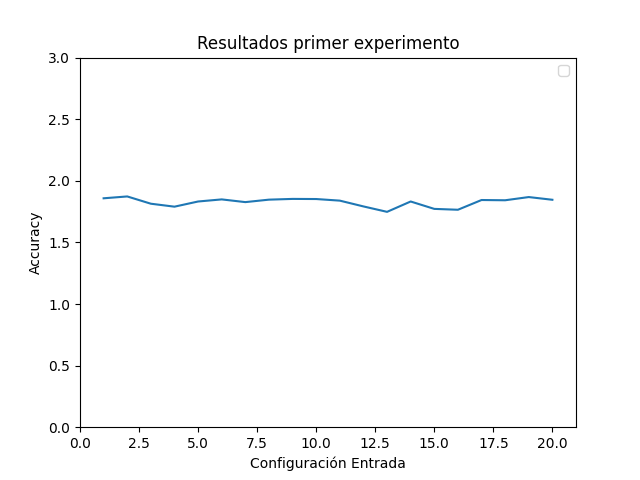
\includegraphics[width=.7\linewidth]{images/resultSecondEval.png}
\caption{Accuracy por ejecución para experimento 3}
\label{fig:westminster_lateral}
\end{subfigure}
\begin{subfigure}[b]{0.60\linewidth}
 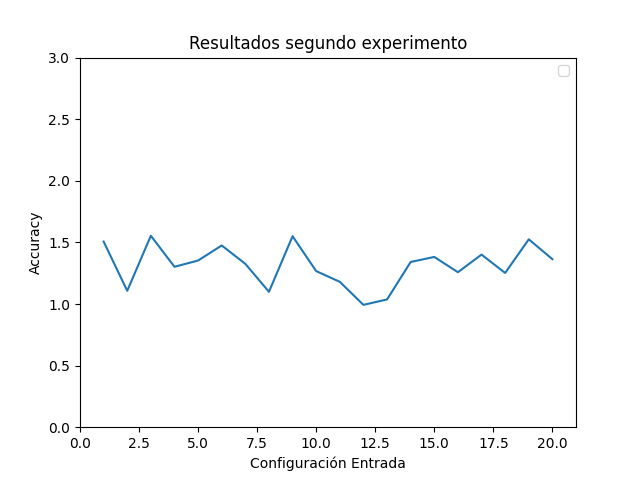
\includegraphics[width=.7\linewidth]{images/resultFourthEval.png}
\caption{Accuracy por ejecución para experimento 4}
\label{fig:accuracy_experiment4_duplicate}
\end{subfigure}
\caption{Accuracy experimentos 3 y 4 (Enfoque 2)}
\label{fig:fitness_exp3_exp4}
\end{figure}



Analizando las salidas para este nuevo enfoque, se observa en el experimento 3 como esta vez las soluciones actuales rompen el dominio anterior dando una mayor gama de soluciones que anteriormente donde en su mayoría las soluciones se basaban todas en una misma configuración. Una de las cosas que se pueden observar y que es un punto común entre la utilización de una función de evaluación y su alternativa es que para la primera forma de ejecución surge la aparición constante de la séptima variable de entrada la cual aparece en todas y cada una de las soluciones mostradas. Tanto con la nueva forma de evaluación como la anterior la aparición de esta variable no cesa. Con esto y como anteriormente se ha comentado, se puede afirmar y reafirmar que cuando esta variable concreta este activa la posibilidad de obtener buenos resultados es bastante alta.

Si además se observa los resultados obtenidos en unos y otros, en el experimento 1 (con la anterior función de evaluación) la media aproximada de los resultados siempre ronda entre 1.9 y 2 de accuracy de la red. Mientras con la nueva función de evaluación reducimos esa media que ahora ronda el 1.80 aproximadamente. A pesar de que esta reducción no es significativa a la hora de buscar las predicciones del potencial hídrico, hace ver como la nueva función de evaluación prioriza configuraciones con mejores respuestas en la red antes que buscar minimizar al máximo el número de variables para después no poder optar a tener una configuración donde las predicciones sean mas satisfactorias y favorables.

Por otro lado, analizando los resultados del experimento 4, se puede observar como la amplia gama de soluciones se mantiene pero esta vez con una diferencia significativa. La gran mayoría de los resultados con la primera función de evaluación en la tabla \ref{tab:experimento1} ronda unos resultados entre el 1.5 y el 2 de accuracy, salvando algunas excepciones. Esta vez con la nueva forma de evaluación esta media se ha reducido pasando a 1 y 1.5 de accuracy aproximadamente, incluso llegando a estar por debajo del 1 en ciertas configuraciones de los operadores genéticos utilizados, dando de nuevo una buena prueba del cambio favorable que ha mostrado la modificación de la función de evaluación, arrojando unos resultados extraordinarios.

\newpage
Para poder observar el comportamiento de las soluciones encontradas, la figura \ref{fig:prediccion_final} representa las predicciones obtenidas por una de las mejores soluciones comparadas con los resultados reales de potencial hídrico que se deben obtener. Se puede observar que el modelo está bien entrenado, obteniendo perdiciones muy próximas al valor esperado. Debemos tener en cuenta la escala del error, que es muy baja, lo que está en sintonía con el accuracy de la red optimizada para el número de variables indicadas por el individuo.

\begin{figure}[h!]
\centering
 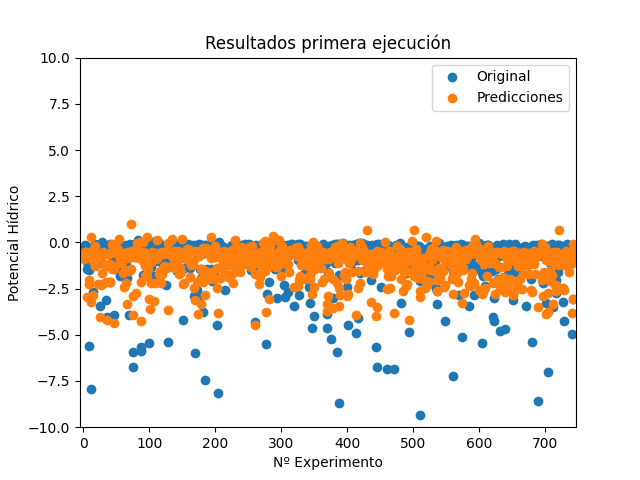
\includegraphics[width=.8\linewidth]{images/Prediccion.png}
\caption{Predicción del individuo 0101000010010}
\label{fig:westminster_aerea}
\end{figure}


